%!TeX encoding = UTF-8
%!TeX program = xelatex
% --------------------------------------------------------
%  欢迎使用桂林电子科技大学本科毕业论文LaTex模板(v3.0)
%    项目:https://github.com/wrm244/GUEThesis
%     请参考项目目录下的docs文件夹额外说明
% --------------------------------------------------------
\special{dvipdfmx:config z 1}
% 修改数值是否压缩,1:压缩,0:不压缩,不压缩会加快编译速度,但会增加PDF体积

\documentclass[eversion]{thesis-guet} 
% documentclass[]参数:eversion:电子版 pversion:打印版
% \usepackage{showframe} % 显示排版框架
% \TPshowboxestrue % 显示textblock 框架,方便调整位置

\definecolor{shadecolor}{RGB}{255,204,75} % 定义高亮颜色
\graphicspath{{./image/},{./image/chapter1/},{./image/chapter2/}}% 图片所在位置

% ----------------------------------------------
%     文章信息
% ----------------------------------------------
\title{桂林电子科技大学毕业论文标题}{} % 题目{中文}{英文}
\author{你的名字}
\advisor{教师名字}   % 导师姓名
\protitle{教授}  % 导师职称.
\school{计算机与信息安全学院}  % 所在学院
\major{你的专业}  % 学科专业或领域
\studentnumber{2000300XXX}  % 学号
\degreecategories{工学学士}  % 申请学位门类或类别
\datereply{\today}  % 可更换为具体日期如:\datereply{2023年5月28日}

% -----------------------------------------------
%     封面
% -----------------------------------------------
\begin{document}
\makecover % 封面
%也可使用另外添加PDF文件作为封面,如盲审封面 \bindpdfcover{盲审学位论文封面(示例).pdf} 
\originalitydeclaration   % 独创性声明
%也可使用已签字的扫面版独创性声明PDF文件 \signatureofdeclaration{./docs/独创性声明(示例).pdf} 
% !Mode:: "TeX:UTF-8"


\begin{chineseabstract}

摘要应概括论文的主要信息,应具有独立性和自含性,即不阅读论文的全文,就能获得必要的信息。摘要内容一般应包括研究目的、内容、方法、成果和结论,要突出论文的创造性成果或新见解,不要与绪论相混淆。语言力求精练、准确,以300-500 字为宜。关键词是供检索用的主题词条,应体现论文特色,具有语义性,在论文中有明确的出处,并应尽量采用《汉语主题词表》或各专业主题词表提供的规范词。关键词与摘要应在同一页,在摘要的下方另起一行注明,一般列 3-5 个,按词条的外延层次排列(外延大的排在前面)。

\chinesekeyword{(关键词一般为5个左右,内容采用小四号、宋体、接排、各关键词之间用分号隔开)}
\end{chineseabstract}

\begin{englishabstract}

The content of the English abstract is the same as the Chinese abstract, 250-400 content words are appropriate. Start another line below the abstract to indicate English.

\englishkeyword{(Keywords 3-5 各关键词之间用分号隔开)}
\end{englishabstract}    % 摘要
\thesistableofcontents       % 目录

% -------------------------------------------------
%    论文各章节(详见目录下chapter文件夹)
% -------------------------------------------------
% !Mode:: "TeX:UTF-8"
%此为引言,因为没有数字标识所以不用书写chapter{引言}。
%[h]为hear代码所在位置,\caption为表注题注,\cref{}引用图表公式章节等,\cite为引用参考文献,\subfloat子图,\label标签,\begin{figure}图片环境,\begin{table}表格环境,\begin{equation}公式环境,\toprule三线表顶线,\cmidrule三线表中线,\bottomrule三线表底线,\begin{theorem}定理,\begin{proof}证明,\begin{corollary}推论,\begin{lemma}引理

随着人工智能和第五代移动通信技术等系统技术的发展\cite{Lau_2022},推动着半导体行业在移动便携设备、高性能计算机、自动驾驶、物联网和大数据等应用领域的发展\cite{Lau_2022},同时也推动着电子芯片向着小型化和高集成化方向发展快速发展\cite{Sadique.Murtaza.ea_2022}。
在过去的几十年里处理器上的晶体管数量依照摩尔定律\cite{Tan.Du.ea_2021}的预测呈现出指数级的增长趋势,如这张50年间的微处理器的发展趋势图(\cref{fig:processor-trend})所示。
……

\chapter{第二章示例}
\begin{figure}[htb]
    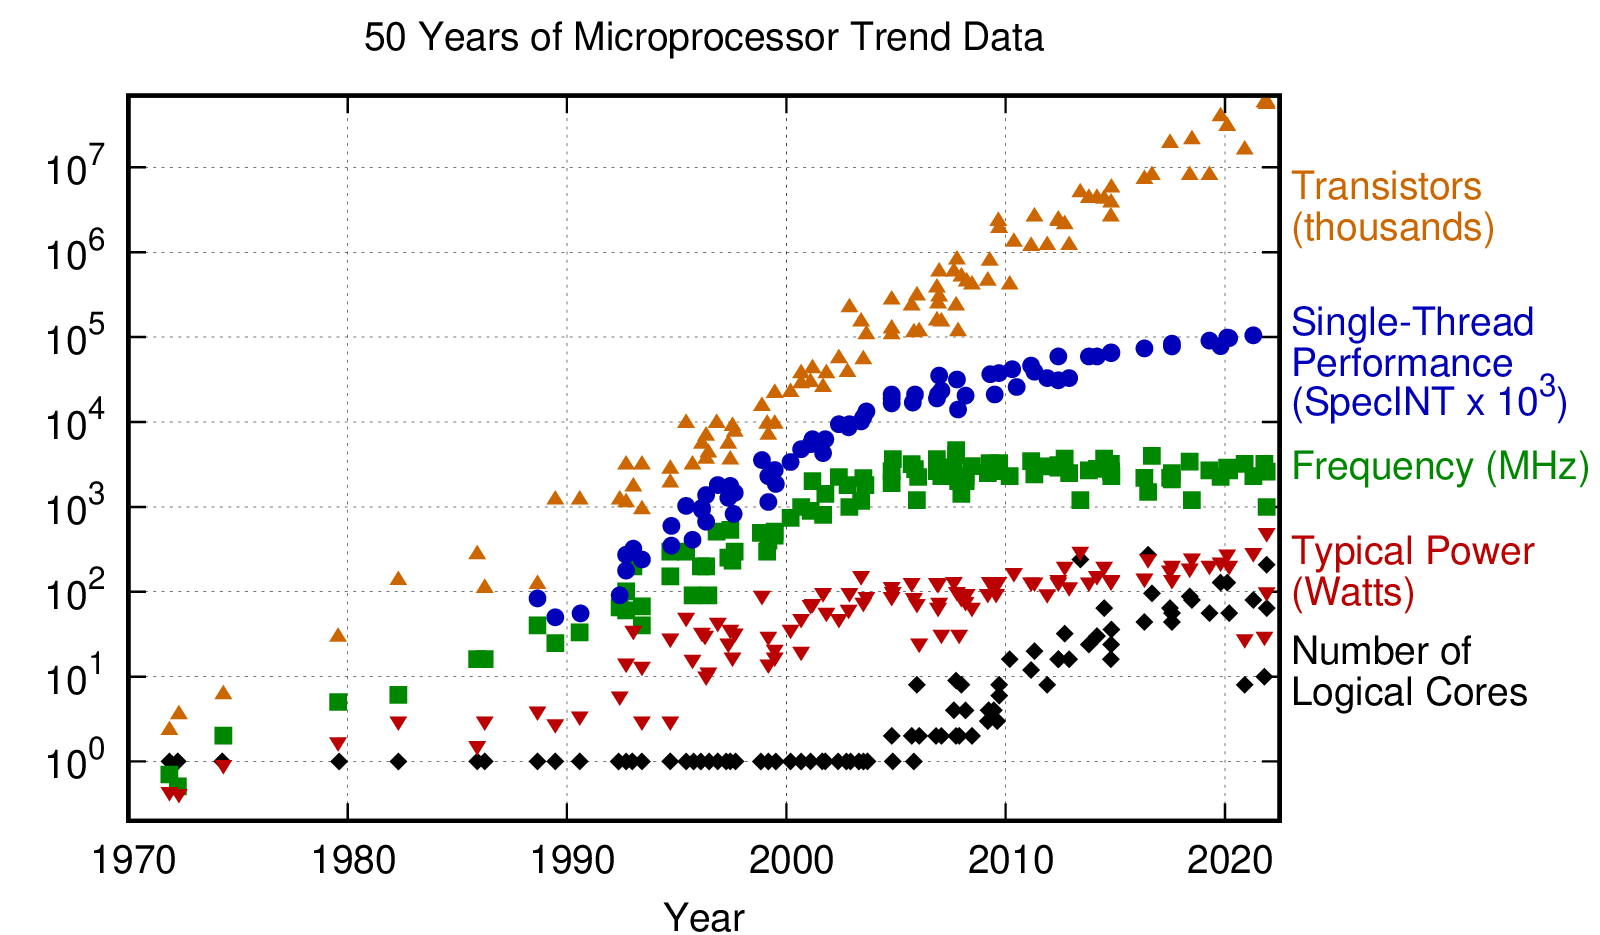
\includegraphics[width=0.8 \textwidth]{50-years-processor-trend.png}
    \caption[处理器发展]{近50年微处理器发展趋势} % 中括号中内容为插图索引中显示内容,可在题注内容过长时使用
    \label{fig:processor-trend}
\end{figure}


同一行中的子图之间要留有空间,不要占满!否则会自动换行!

子图之间空一行表示换行。

\begin{figure}[htb]
    \subfloat[改进前的结构]{
        \label{fig:Unimproved-cooling-structure}
        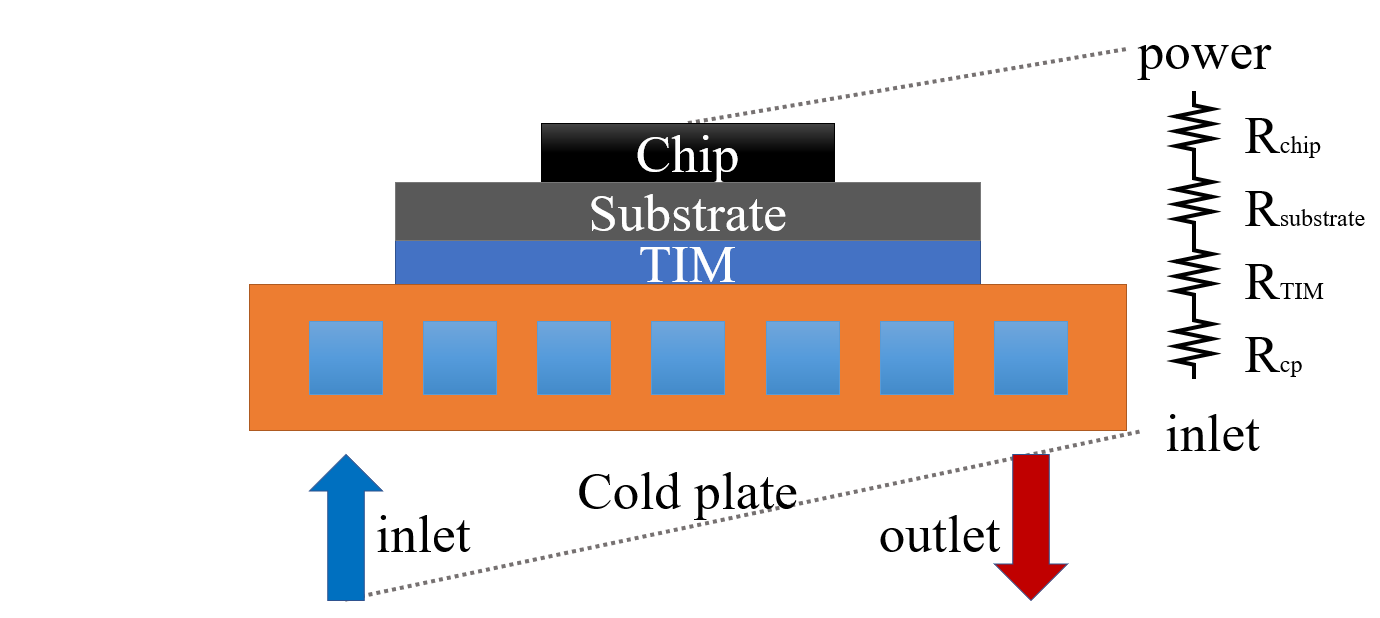
\includegraphics[width=0.45\linewidth]{Unimproved-cooling-structure.png}}
    \subfloat[基板内进行微通道散热]{
        \label{fig:LTCC-Microchannels}
        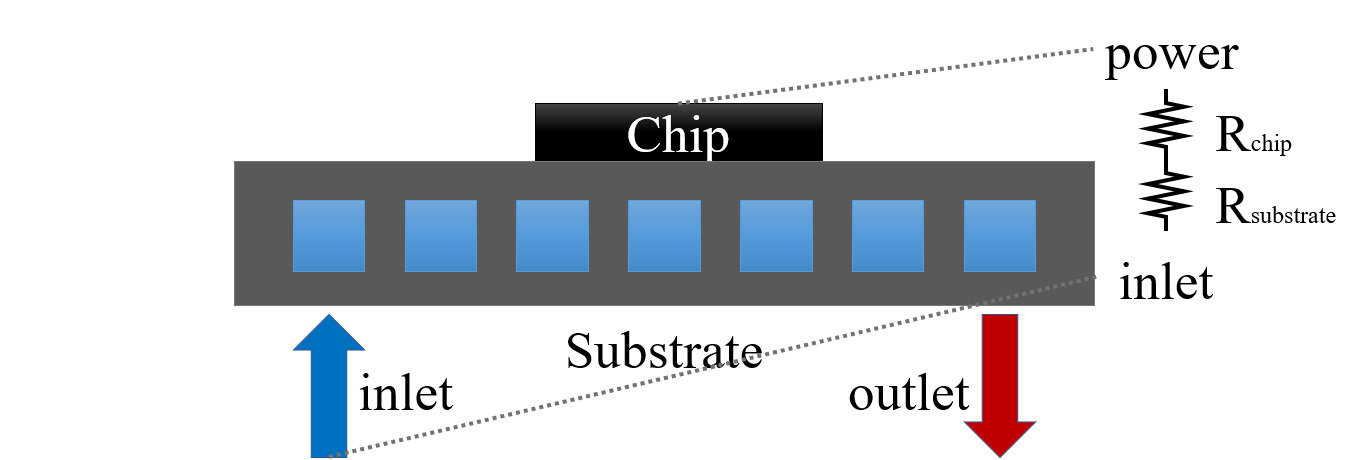
\includegraphics[width=0.45\linewidth]{LTCC-Microchannels.png}}

    \subfloat[嵌入散热模块]{
        \label{fig:Embedded-cooling-module}
        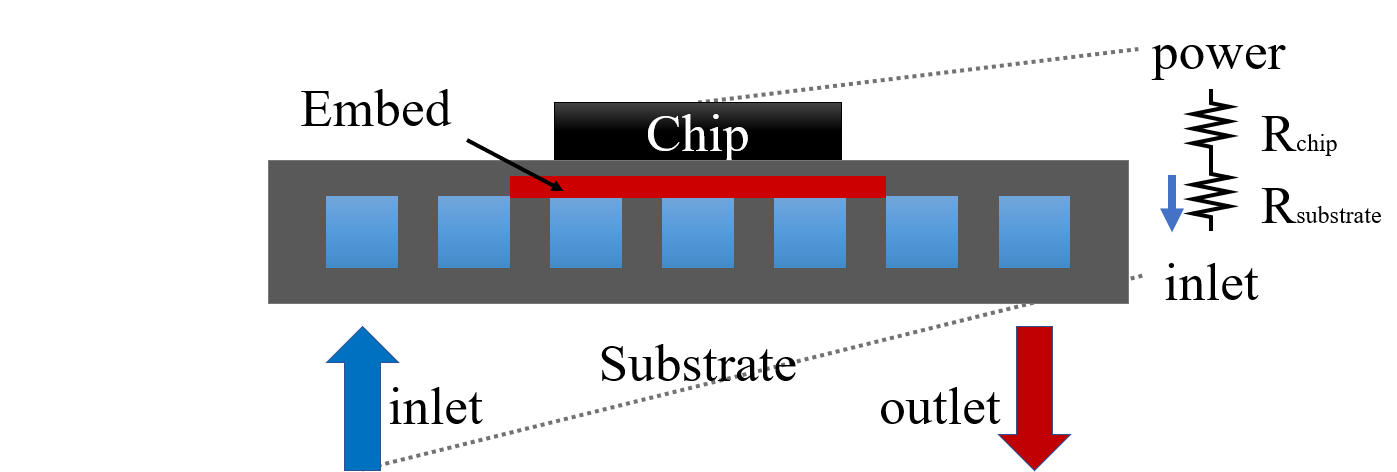
\includegraphics[width=0.45\linewidth]{Embedded-cooling-module.png}}
    \subfloat[带针鳍或肋的嵌入式散热模块]{
        \label{fig:Rib-pin-fin}
        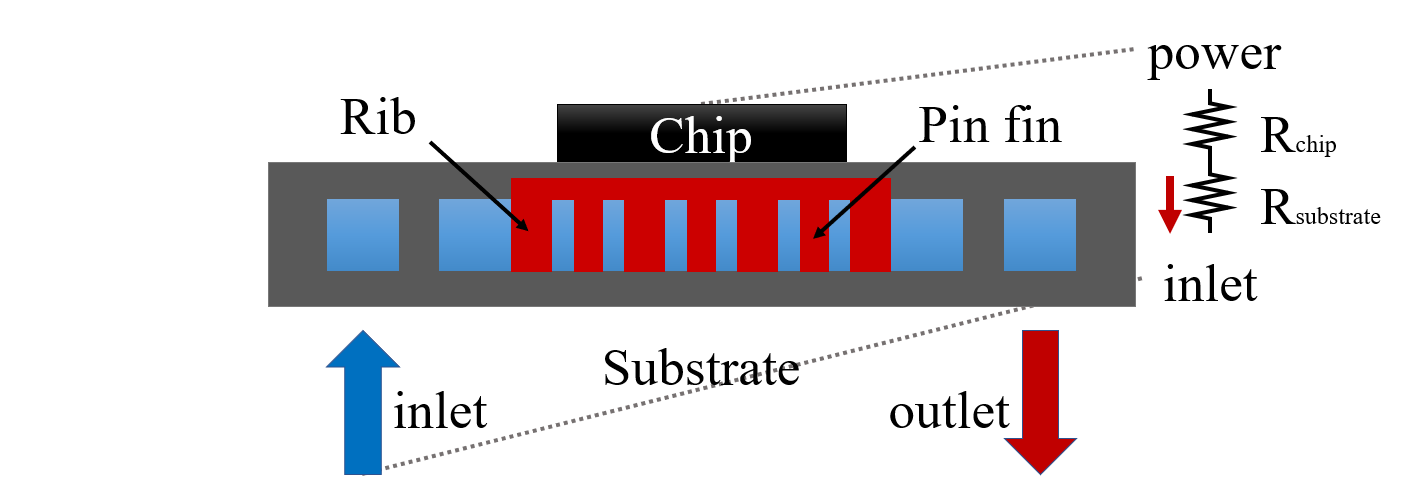
\includegraphics[width=0.45\linewidth]{Rib-pin-fin.png}}
    \caption{三种强化传热途径示意图}
    \label{fig:Three-enhanced-heat-transfer-paths}
\end{figure}



\cref{ch:2}:相关理论基础及结构设计要求与思路。本章主要分为……。

\cref{ch:3}:基于嵌入式散热模块的微通道流动与传热性能研究。本章研究了几种……。

\cref{ch:4}:基于嵌入式散热模块的微通道多目标优化分析。本章在\cref{ch:3}完成基于……。

\cref{ch:5}: 基于MC-RPF的多热源散热结构设计分析及压降优化。本章在\cref{ch:4}完成MC-RPF多目标优化……。

\cref{ch:6}:全文总结与展望。本次研究工作进行总结,并根据全文研究过程中……。



% !Mode:: "TeX:UTF-8"
%此为章节二模板
%\chapter、\section、\subsection、\subsubsection分别对应一二三四级标题
\chapter{表格示例}\label{ch:2}

可使用excel绘制表格,然后粘贴到以下网站中生成latex表格代码。

推荐网站如下:

https://www.tablesgenerator.com/

https://www.latex-tables.com/

\section{普通三线表示例}
普遍学者认为,微通道指的是水力直径在 $10\ \rm{\mu m}$ 到 $1000\ \rm{\mu m}$ 范围内的通道(也有观点认为是 $1\ \rm{\mu m}$ 到 $100\ \rm{\mu m}$)所构成的换热器。
以下是较为常见的微通道尺寸分类,可以参见\cref{tab:division-of-microchannels}。
\begin{table}[htbp]
    \caption[微通道的划分]{微通道的划分\cite{LuSiHong_2021}}
    \setlength{\tabcolsep}{14mm}{ % 因表格过窄,手动设置宽度为7mm
        \begin{tabular}{lc}
            \toprule
            通道种类    & 水力直径$\mu m$   \\
            \midrule
            分子纳米通道  & $\le 0.1$     \\
            过渡性纳米通道 & $0.1\sim 1$   \\
            过渡性微通道  & $1\sim 10$    \\
            微通道     & $10\sim 1000$ \\
            常规通道    & $>1000$       \\
            \bottomrule
        \end{tabular}}
    \label{tab:division-of-microchannels}
\end{table}



\section{跨页表格示例}

\begin{longtable}{@{\extracolsep{\fill}}cccccc@{}}  \\
    \caption{RSM仿真实验规划表}
    \label{tab:Experimental-Planning}  \\
    \toprule
    标准序 & 运行序 & $H_{rib}\ \rm{(mm)}$ & $H_{pf}\ \rm{(mm)}$ & $N_{pf}$ & $N_{ac}$ \\ \midrule
    \endfirsthead
    %
    \multicolumn{6}{c}%
    {\fontsize{10.5pt}{10.5pt}\selectfont\heiti{表 \thetable\ RSM仿真实验规划表 (续)}} \\
    \toprule
    标准序 & 运行序 & $H_{rib}\ \rm{(mm)}$ & $H_{pf}\ \rm{(mm)}$ & $N_{pf}$ & $N_{ac}$ \\ \midrule
    \endhead
    %
    \bottomrule
    \endfoot
    %
    \endlastfoot
    %
    11  & 1   & 0.16            & 0.8            & 6        & 16       \\
    13  & 2   & 0.16            & 0.16           & 22       & 16       \\
    15  & 3   & 0.16            & 0.8            & 22       & 16       \\
    12  & 4   & 0.8             & 0.8            & 6        & 16       \\
    10  & 5   & 0.8             & 0.16           & 6        & 16       \\
    2   & 6   & 0.8             & 0.16           & 6        & 0        \\
    19  & 7   & 0.48            & 0.48           & 14       & 8        \\
    1   & 8   & 0.16            & 0.16           & 6        & 0        \\
    20  & 9   & 0.48            & 0.48           & 14       & 8        \\
    18  & 10  & 0.48            & 0.48           & 14       & 8        \\
    8   & 11  & 0.8             & 0.8            & 22       & 0        \\
    14  & 12  & 0.8             & 0.16           & 22       & 16       \\
    6   & 13  & 0.8             & 0.16           & 22       & 0        \\
    17  & 14  & 0.48            & 0.48           & 14       & 8        \\
    7   & 15  & 0.16            & 0.8            & 22       & 0        \\
    16  & 16  & 0.8             & 0.8            & 22       & 16       \\
    4   & 17  & 0.8             & 0.8            & 6        & 0        \\
    9   & 18  & 0.16            & 0.16           & 6        & 16       \\
    5   & 19  & 0.16            & 0.16           & 22       & 0        \\
    3   & 20  & 0.16            & 0.8            & 6        & 0        \\
    25  & 21  & 0.48            & 0.48           & 6        & 8        \\
    22  & 22  & 0.8             & 0.48           & 14       & 8        \\
    23  & 23  & 0.48            & 0.16           & 14       & 8        \\
    29  & 24  & 0.48            & 0.48           & 14       & 8        \\
    28  & 25  & 0.48            & 0.48           & 14       & 16       \\
    30  & 26  & 0.48            & 0.48           & 14       & 8        \\
    26  & 27  & 0.48            & 0.48           & 22       & 8        \\
    27  & 28  & 0.48            & 0.48           & 14       & 0        \\
    21  & 29  & 0.16            & 0.48           & 14       & 8        \\
    24  & 30  & 0.48            & 0.8            & 14       & 8        \\ \bottomrule
\end{longtable}

\section{本章小节}
本章介绍了基于嵌入式散热模块的微通道散热技术所涉及的基……
% !Mode:: "TeX:UTF-8"

\chapter{数学公式示例}\label{ch:3}

\section{公式示例}
在本次研究中应用到计算流体动力学(Computational Fluid Dynamics,CFD)对研究对象进……。


\subsection{普通带序号公式}
\begin{equation}
    \frac{\partial u}{\partial x}+\frac{\partial v}{\partial y}+\frac{\partial v}{\partial z}=0
\end{equation}
u,v,w 分别是 x,y,z 方向的速度分量。


\subsection{需要对齐的多个带序号的公式}

\&号为对其对齐标记最好放置在计算符号之前,如=、+、-之前;

\textbackslash\textbackslash 表示换行。

\begin{align}% 式中的&为对齐的位置标记
    u & \frac{\partial u}{\partial x}+v \frac{\partial u}{\partial y}+w \frac{\partial u}{\partial z}=-\frac{1}{\rho_{f}} \frac{\partial p}{\partial x}+\frac{\mu_{f}}{\rho_{f}}\left(\frac{\partial^{2} u}{\partial x^{2}}+\frac{\partial^{2} u}{\partial y^{2}}+\frac{\partial^{2} u}{\partial z^{2}}\right) \\
    u & \frac{\partial v}{\partial x}+v \frac{\partial v}{\partial y}+w \frac{\partial v}{\partial z}=-\frac{1}{\rho_{f}} \frac{\partial p}{\partial y}+\frac{\mu_{f}}{\rho_{f}}\left(\frac{\partial^{2} v}{\partial x^{2}}+\frac{\partial^{2} v}{\partial y^{3}}+\frac{\partial^{2} v}{\partial z^{3}}\right) \\
    u & \frac{\partial w}{\partial x}+v \frac{\partial w}{\partial y}+w \frac{\partial w}{\partial z}=-\frac{1}{\rho_{f}} \frac{\partial p}{\partial z}+\frac{\mu_{f}}{\rho_{f}}\left(\frac{\partial^{2} w}{\partial x^{2}}+\frac{\partial^{2} w}{\partial y^{2}}+\frac{\partial^{2} w}{\partial z^{2}}\right)
\end{align}
$\rho_{f}$ 和 $\mu_{f}$ 分别是冷却剂的密度和动态粘度,p 是冷却剂压力。


\subsection{需要换行对齐的长公式}

\begin{equation}\label{eq:P}
    \begin{split}
        f_3 & = 6.272 + 3.02 H_{rib} + 6.08 H_{pf} + 0.0368 N_{pf} - 0.8848 N_{ac} + 0.04381 N_{ac}^2\\
        & + 6.35 H_{rib} \times H_{pf} - 0.3602 H_{rib}\times N_{ac} - 0.5497 H_{pf}\times N_{ac}
    \end{split}
\end{equation}

\subsection{其他公式示例}
\begin{equation}
    \begin{aligned}
    \left\{
        \begin{array}{l}
        \text {find}\enspace H_{rib},H_{rib},N_{pf},N_{ac} \\
        \text {min} \enspace F(H_{rib},H_{rib},N_{pf},N_{ac})= min\{f_1,f_2,f_3\} \\

            \text{s.t.\enspace}\enspace 0.2 \leqslant H_{rib} \leqslant 0.8    \\
            \hspace{2.2em} 0.2 \leqslant H_{pf} \leqslant 0.8                     \\
            \hspace{2.2em} 6 \leqslant N_{pf} \leqslant 22,\ N_{pf}\in \mathbb{O} \\
            \hspace{2.2em} 0 \leqslant N_{ac} \leqslant 16,\ N_{ac}\in \mathbb{E}
        \end{array}
    \right. 
    \end{aligned}
    \label{eq:MO}
\end{equation}
% !Mode:: "TeX:UTF-8"

\chapter{列表与符号示例}\label{ch:4}

\section{概述}
本章在\cref{ch:3}完成基……。

\section{列表示例}\label{sec:enumerate}

\subsection{普通列表示例}
\begin{enumerate}
    \item 在基板内部进行微通道散热以缩短传热路径,见\cref{fig:LTCC-Microchannels};
    \item 在基板内嵌入散热模块减少整体热阻,提高热传导效率,见\cref{fig:Embedded-cooling-module};
    \item 在嵌入式散热模块上制作针鳍或肋增强对流传热,以进一步减小热阻,见\cref{fig:Rib-pin-fin}。
\end{enumerate}

\subsection{标号为阿拉伯数字的列表}

\begin{enumerate}[label =(\arabic*)]

    \item 基于嵌入式散热模块的微通道流动与传热性能研究。
          将三种带有嵌入式散热模块的微通道:带有针鳍……
          最终选用MC-RPF作为核心散热结构;
    \item 分析几何参数对带有针鳍-肋嵌入式散热模块微通道流动与传热的影响。
          主要研究……;
    \item 对采用针鳍-肋嵌入式散热模块的微通道进行多目标优化。
          采用响应面分析法(Response Surface Methodology,RSM)与……;
    \item 基于MC-RPF的多热源散热结构设计分析。
          为解决在多热源应……;
    \item 基于MC-RPF的多热源散热结构压降优化。
          以压降损失相关理论为指导依据,……。

\end{enumerate}

\subsection{自定义列表标号}
\noindent NSGA-Ⅱ具体操作步骤如下:
\begin{enumerate}[leftmargin = 6em, labelsep = 0em]
    \item[步骤一、] 随机生成初始化种群,设置代数$Gen = 0$;
    \item[步骤二、] 判断是否生成第一代种群,如已生成则令其代数$Gen = 2$,否则进行快速非支配排序、选择、SBX、PM生成第一代子群,并设置代数$Gen = 2$;
    \item[步骤三、] 将父代与子代的种群进行合并形成新的父代种群;
    \item[步骤四、] 判断是否生成新的父代种群,如果未生成则进行快速非支配排序、拥挤度计算、精英策略选择操作以生成新的父代;
    \item[步骤五、] 对新生成的父代进行选择、SBX、PM操作生成新子群;
    \item[步骤六、] 判断当前代数是否小于设置的最大代数,若小于设置的最大代数则返回步骤三进行循环,否则,NSGA-Ⅱ结束运行。
\end{enumerate}

\section{本章小节}
\section{空白符号}
    % 空行分段,多个空行等同于一个
    % 自动缩进,绝对不能使用空行代替
    % 英文中多个空格处理为一个空格,中文中空格会被忽略
    % 汉字与其他字符的间距会自动有XeLaTeX处理
    % 禁止使用中文全角空格
 
    % 1em(当前字体中M的宽度)
    1em: a\quad b
 
    % 2em
    2em: a\qquad b
 
    % 约为1/6个em
    1/6个em: a\,b 或 a\thinspace b
 
    % 0.5个em
    0.5个em: a\enspace b
 
    % 空格
    空格: a\ b
 
    % 硬空格,即不能分割的空格
    硬空格: a~b
 
    % 1pc=12pt=4.218mm
    指定宽度1pc: a\kern 1pc b
 
    指定宽度-1em: a\kern -1em b
 
    指定宽度1em: a\hskip 1em b
 
    指定宽度35pt: a\hspace{35pt}b
 
    % 占位宽度
    占位宽度为xyz: a\hphantom{xyz}b

\section{\LaTeX 控制符}
\#              % 输出井号
\$              % 输出美元符号
\{ \}           % 输出大括号
\~{}            % 输出波浪
\_{}            % 输出下划线
\^{}            % 输出尖角
\textbackslash  % 输出反斜杠
\&              % 输出与符号
% !Mode:: "TeX:UTF-8"

\chapter{算法与定理示例}\label{ch:5}

\section{算法示例}

\noindent 算法示例如下:

\begin{algorithm}[H]
    \KwData{this text}
    \KwResult{how to write algorithm with \LaTeX2e}
    initialization\;
    \While{not at end of this document}{
        read current\;
        \eIf{understand}{
            go to next section\;
            current section becomes this one\;
        }{
            go back to the beginning of current section\;
        }
    }
    \caption{How to wirte an algorithm.}
\end{algorithm}


\section{定理定义的使用示例}
\begin{theorem}
如果时域混合场积分方程是时域电场积分方程与时域磁场积分方程的线性组合。
\end{theorem}
\begin{proof}
由于时域混合场积分方程是时域电场积分方程与时域磁场积分方程的线性组合,因此时域混合场积分方程时间步进算法的阻抗矩阵特征与时域电场积分方程时间步进算法的阻抗矩阵特征相同。
\end{proof}
\begin{corollary}
时域积分方程方法的研究近几年发展迅速,在本文研究工作的基础上,仍有以下方向值得进一步研究。
\end{corollary}
\begin{lemma}
因此时域混合场积分方程时间步进算法的阻抗矩阵特征与时域电场积分方程时间步进算法的阻抗矩阵特征相同。
\end{lemma}   % 可根据需求自行添加章节数
% !Mode:: "TeX:UTF-8"

\chapter{全文总结与展望}\label{ch:6}
内容主要为:概括研究结果,指出其创新处和价值点;指出本设计(论文)未研究或不足之处;对事物发展或研究领域研究发展的展望
\section{全文总结}

\section{后续工作展望} % 总结与展望
% --------------------------------------------------
%     参考文献
% --------------------------------------------------
\thesisbibliography{./references/reference.bib} % 参考文献
%当参考文献数目超过100时,可以使用large选项调整编号\thesisbibliography{large}{./references/reference.bib} 

% ---------------------------------------------------------------
% 此处一般不用,除非要自定义参考文献样式,更换参考文献样式文件
% \bibliographystyle{thesis-guet(base-gbt7714-numerical)}  % 自定义参考文献样式
% \bibliography{reference} % 参考文献库
% ---------------------------------------------------------------

\thesisacknowledgement  % 致谢
\normalfont
\end{document}
